
\subsection{Analyse HVV Hamburger Verkehrsverbund GmbH}
Bei der HVV ist der fehlende Kontrast von Text zu Hintergrund der häufigste Fehler. Die Primärfarbe ist ein Rot, welches auf weiß nicht auseichend gut zu erkennen ist. Da viele Elemente in dem Rot gehalten sind, treten auch viele Fehler auf der Website auf. Damit wurde das Kriterium 1.4.3 "Mindestkontrast" nicht eingehalten.
\begin{figure}[H]
    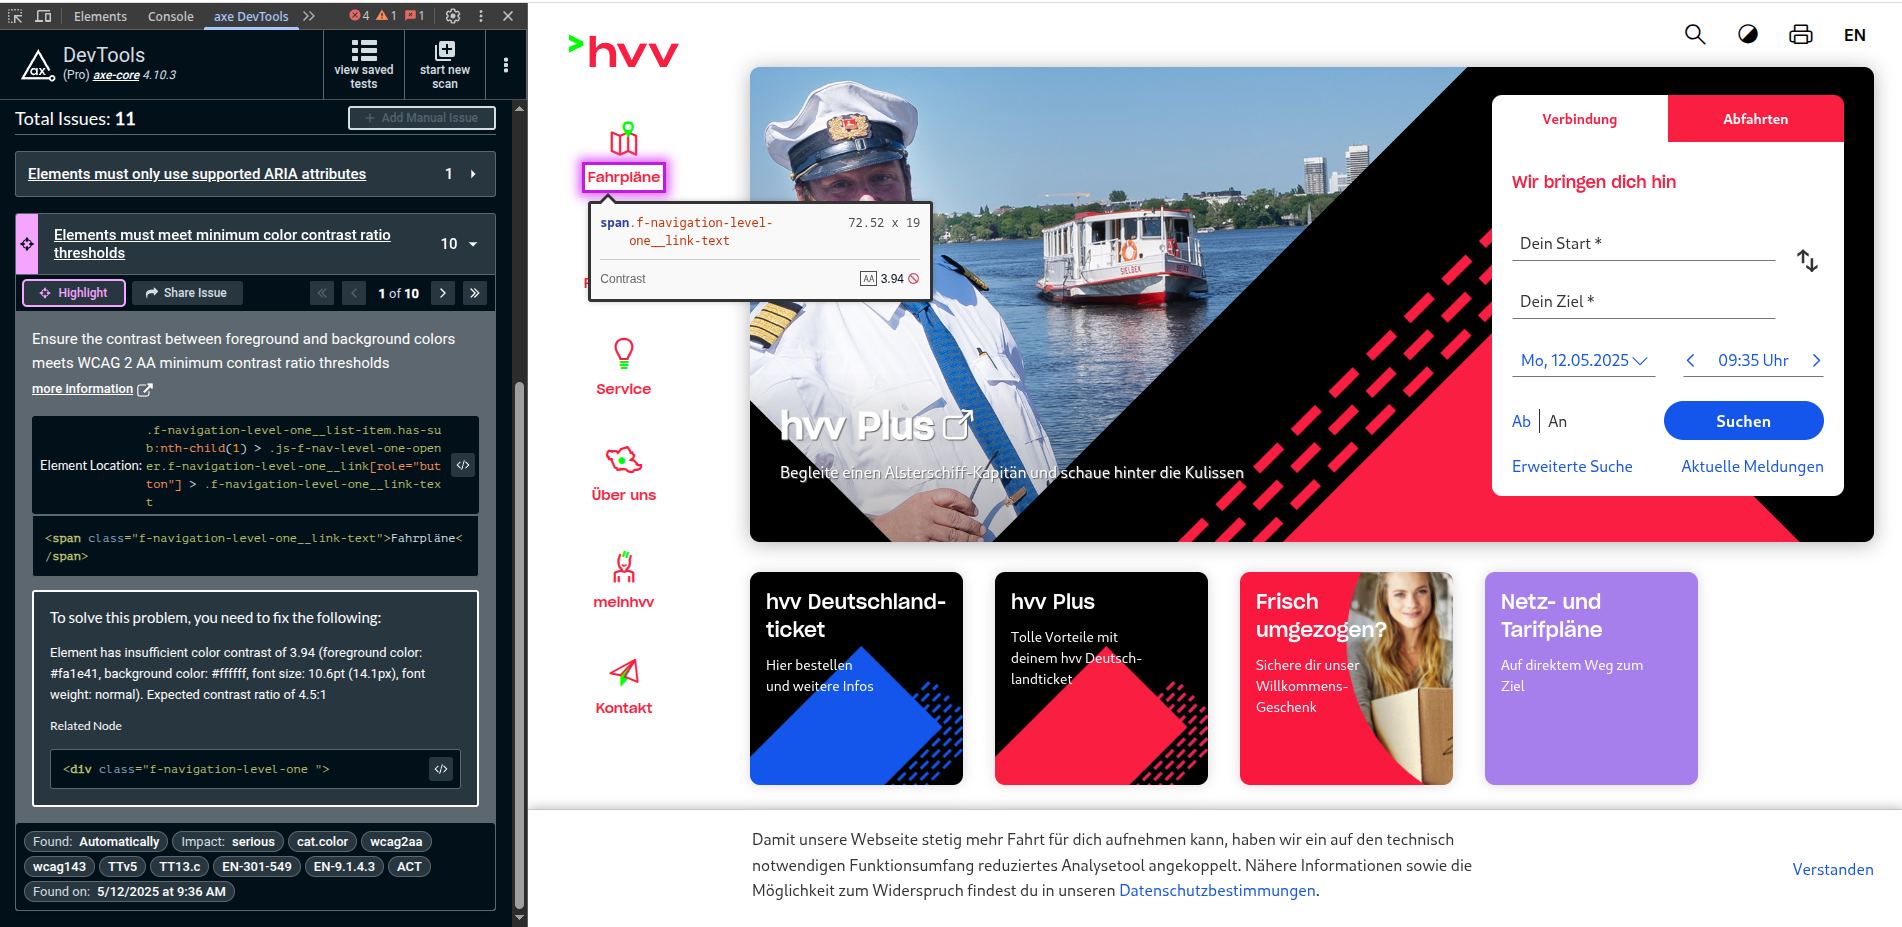
\includegraphics[width=\textwidth]{img/hvv_failed-minimum-contrast.png}
    \caption{Kontrastprobleme auf der Startseite}
\end{figure}
Auch bei der Tastaturbedienbarkeit sind auf der Seite einige Fehler aufgetreten. So ist es nicht möglich, den Button \enquote{Eingabe löschen} in dem Routenplaner zu klicken. Es besteht immer noch die Möglichkeit, den Text manuell zu löschen, aber der Button erfüllt nicht seinen Zweck. Dies ist ein Verstoß gegen Kriterium 2.1.1 "Tastaturbedienbarkeit".
\begin{figure}[H]
    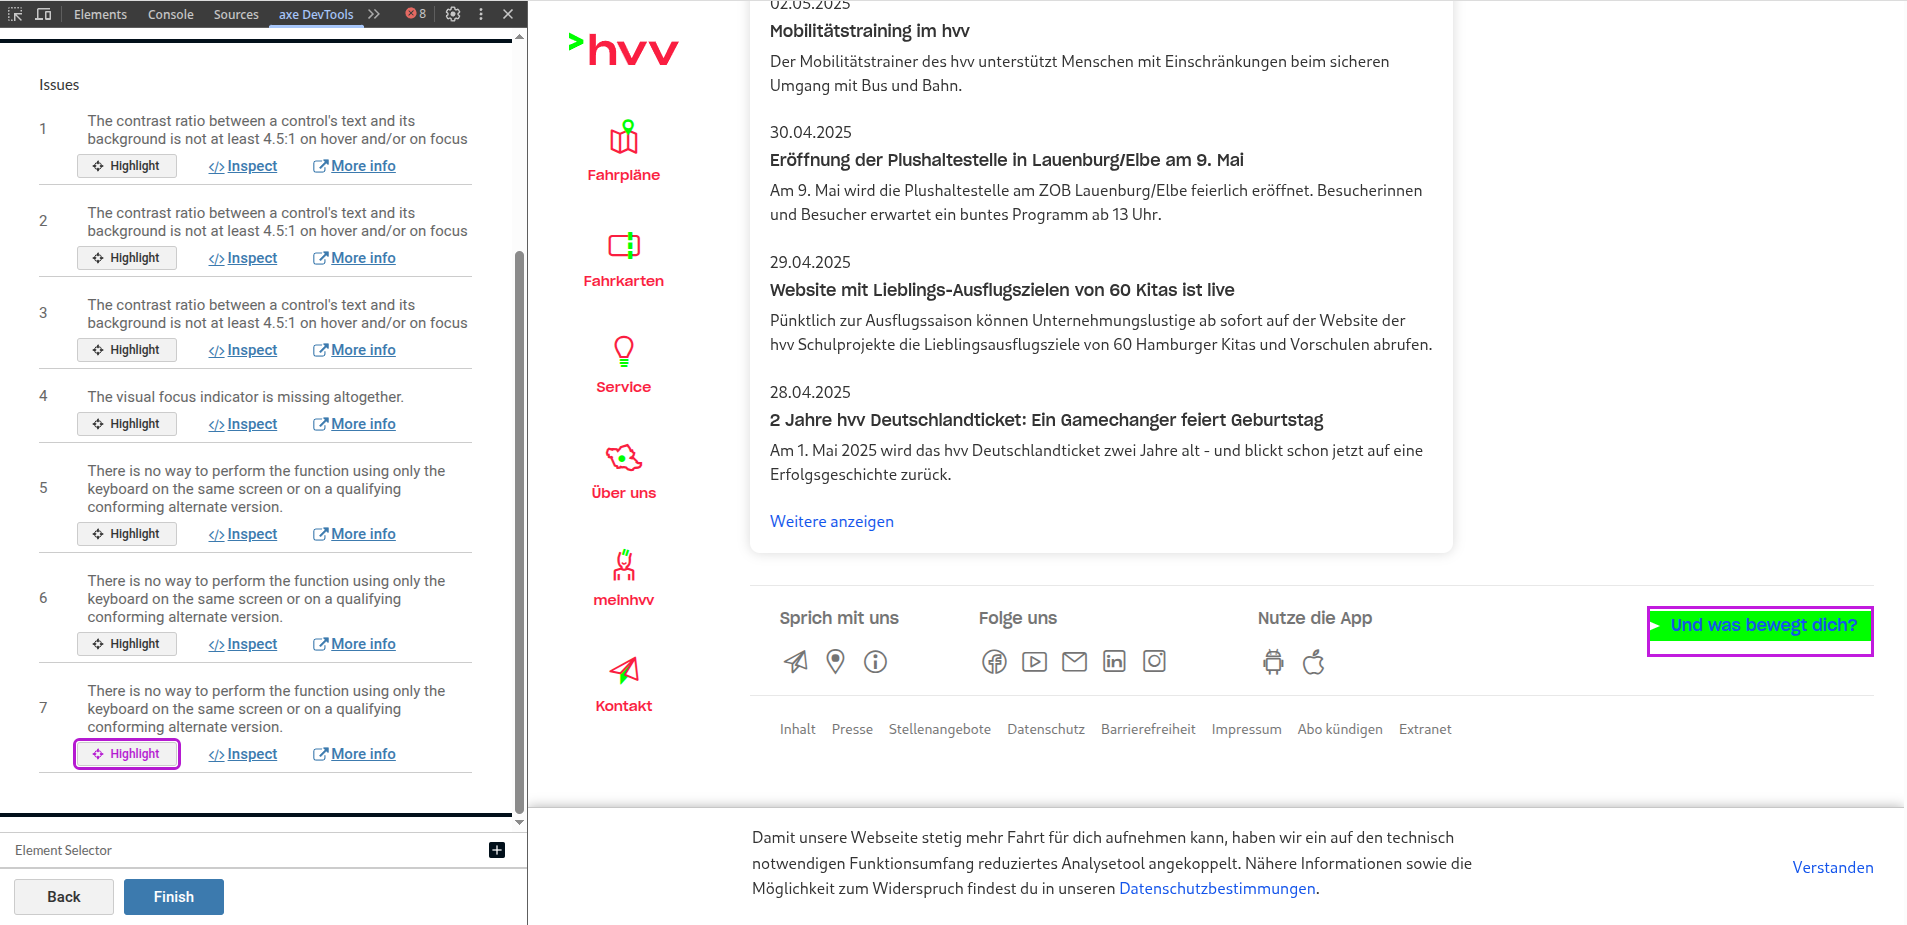
\includegraphics[width=\textwidth]{img/hvv_no-perform-only-keyboard.png}
    \caption{Button ohne Tastaturbedienbarkeit}
\end{figure}

Zusätzlich ist bei dem \enquote{Suchen}-Button kein visueller Fokus gegeben. Es wurde beim Fokussieren nur ein Schlagschatten verwendet, der kaum zu erkennen ist. Das reicht als visueller Fokus nicht aus und verletzt das Kriterium 2.4.7 "Fokus sichtbar".

\begin{figure}[H]
    \centering
    \begin{minipage}[t]{0.49\textwidth}
        \centering
        
\includegraphics[width=\textwidth]{img/hvv_button-without-focus.png}
        \caption{Button ohne Fokus}
    \end{minipage}
    \hfill
    \begin{minipage}[t]{0.49\textwidth}
        \centering
        
\includegraphics[width=\textwidth]{img/hvv_button-with-focus.png}
        \caption{Button mit Fokus}
    \end{minipage}
\end{figure}

Auch die Links sind nicht korrekt umgesetzt. Das Kriterium 1.4.1 \enquote{Verwendung von Farben} sieht vor, dass Links auch ohne Farben funktionieren müssen. Da einige Links sich aber nur durch die Farbe von dem restlichen Text unterscheiden, ist dies nicht gegeben.

\begin{figure}[H]
    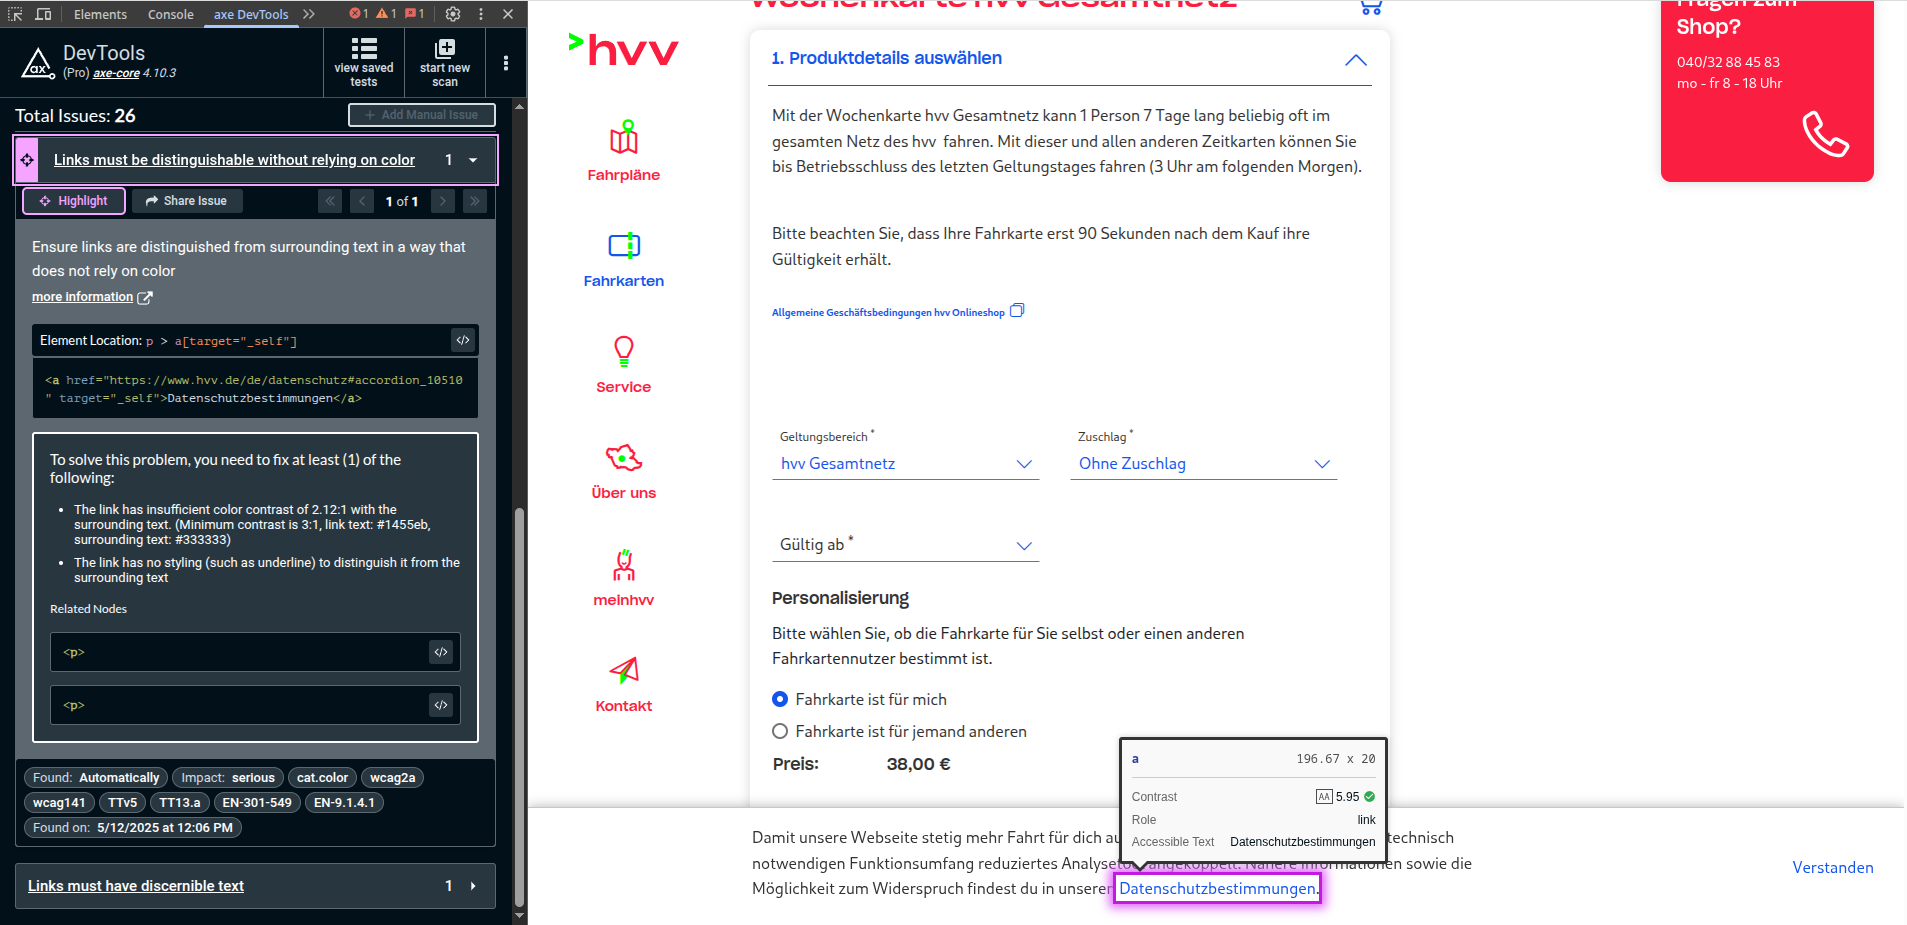
\includegraphics[width=\textwidth]{img/hvv_links-not-only-rely-on-color.png}
    \caption{Link nur durch Farbe unterschieden}
\end{figure}

Beim Kauf eines Tickets fehlen bei den Inputs teilweise auch die Labels. Während die Eingabefelder für den Geltungsbereich und Zuschlag korrekt mit Labels versehen sind, fehlt das Label bei dem Eingabefeld für die Gültigkeit ab einem angegebenen Datum. Dies ist ein Verstoß gegen Kriterium 4.1.2 "Name, Rolle, Wert".
\begin{figure}[H]
    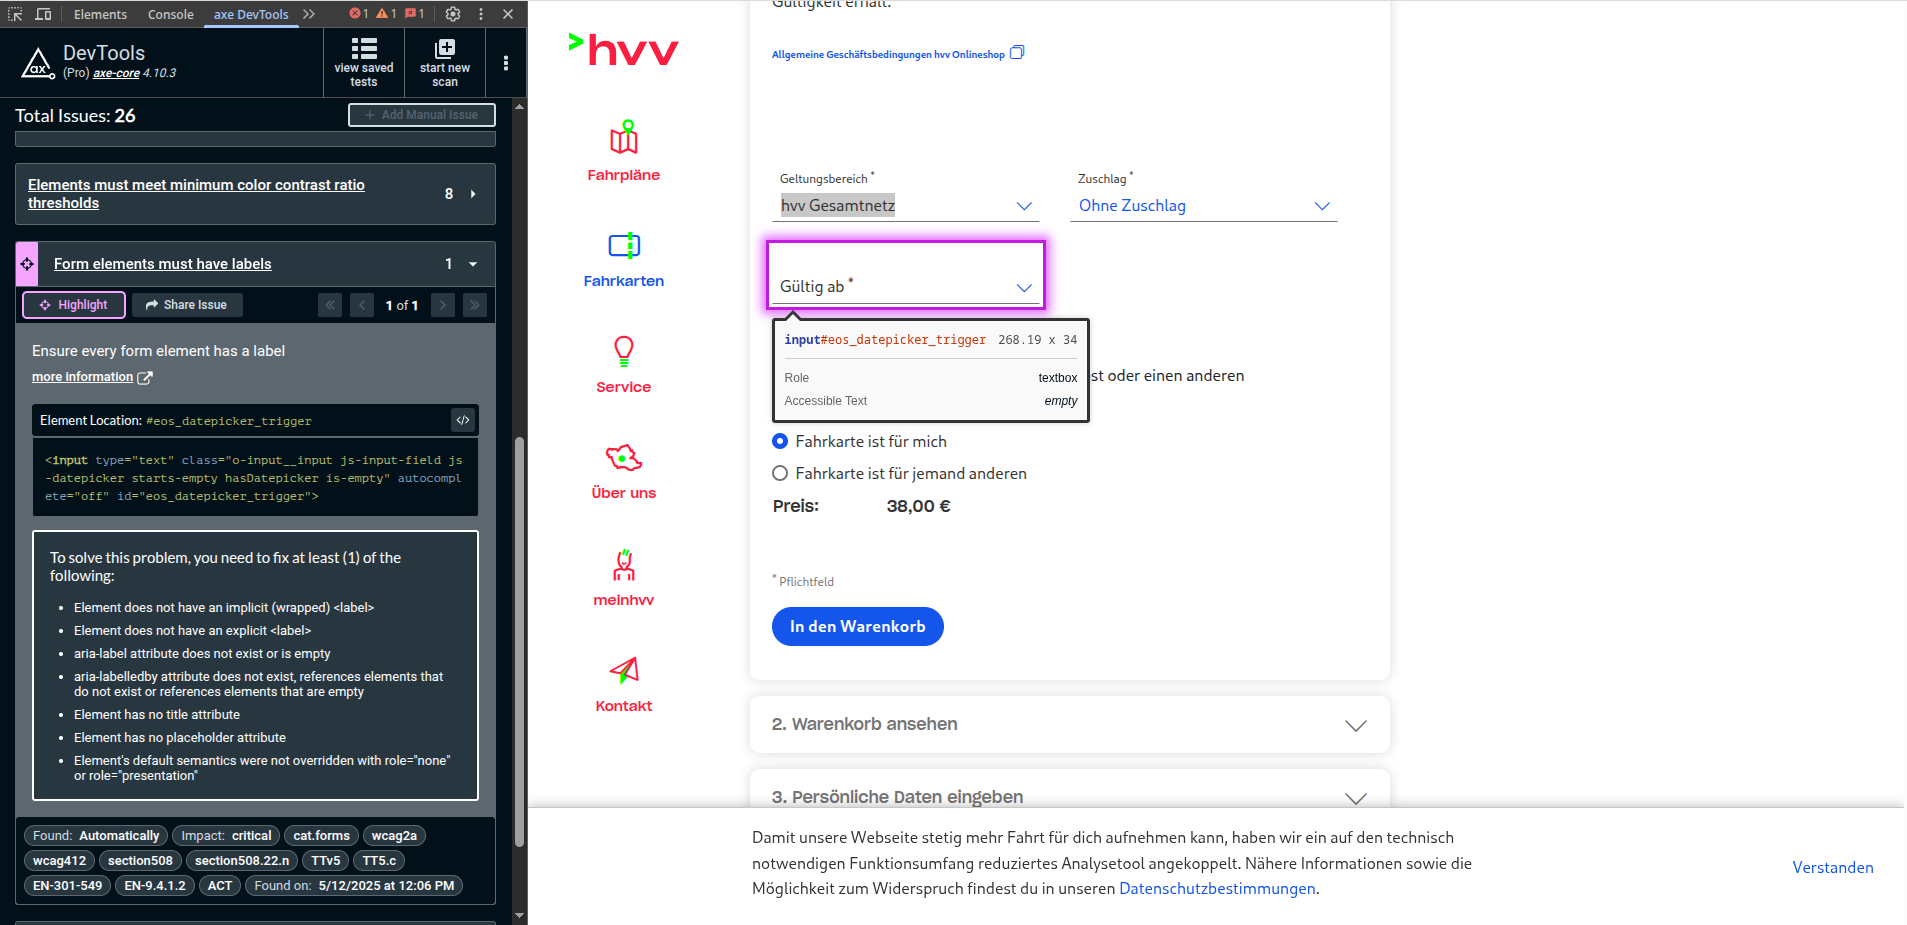
\includegraphics[width=\textwidth]{img/hvv_no-label.png}
    \caption{Fehlendes Label bei einem Eingabefeld}
\end{figure}

Insgesamt sind die Fehler pro Kriterium eher niedrig, allerdings gibt es viele Kriterien, die nicht eingehalten worden sind. Besonders ausschlaggebend waren die Kontrastfehler, da sehr viel Text in dem schlecht sichtbaren Rot gehalten ist.

\begin{figure}[H]
\begin{tikzpicture}
\begin{axis}[
    width=\textwidth,
    height=10cm,
    ybar,
    bar width=12pt,
    xlabel={WCAG-Kriterium},
    ylabel={Fehleranzahl},
    symbolic x coords={ 9.1.1.1, 9.1.3.1, 9.1.4.3, 9.2.1.1, 9.2.4.4, 9.2.4.6, 9.2.4.7, 9.3.3.2, 9.4.1.2 },
    xtick=data,
    x tick label style={rotate=45, anchor=east},
    ymin=0,
    ymax=300,
    enlarge x limits=0.1,
    legend style={cells={anchor=west}, legend pos=north east},
    nodes near coords,
    nodes near coords style={font=\scriptsize},
]
\addplot table[x=WCAG-Kriterium,y=Fehleranzahl_axe,col sep=tab] {csv/output/wcag_analyse_HVV_xxxx.csv};
\addplot table[x=WCAG-Kriterium,y=Fehleranzahl_WAVE,col sep=tab] {csv/output/wcag_analyse_HVV_xxxx.csv};
\legend{axe,WAVE}
\end{axis}
\end{tikzpicture}
\caption{Auswertung Analyse HVV}
\end{figure}
